\documentclass[12pt]{beamer}

%CORE PACKAGES---------------------------------
\usepackage{amsmath, amssymb, graphicx, booktabs, tabularx, setspace, soul}
\usepackage{subcaption}
\usepackage{tikz, pgfplots}
\pgfplotsset{compat=1.18}
\usetikzlibrary{positioning, arrows.meta, arrows.meta, positioning, shapes, calc}
\usepackage[many]{tcolorbox}
\usepackage[ruled,vlined]{algorithm2e}
\usepackage{minted}

%FONTS & STYLING-------------------------------
\usepackage{fontspec}
\usefonttheme{professionalfonts}
\setsansfont[
UprightFont     = *Light,
BoldFont        = *Bold,
ItalicFont      = *Light Italic,
BoldItalicFont  = *Bold Italic,
Ligatures       = TeX,
Scale           = MatchLowercase
]{Frutiger LT Pro}
\renewcommand{\familydefault}{\sfdefault}
\linespread{1.}\selectfont
\hyphenpenalty=10000
\exhyphenpenalty=10000

%COLORS & THEMES-------------------------------
\definecolor{aggiemaroon}{RGB}{80,0,0}
\definecolor{beamer@blendedblue}{RGB}{80,0,0}
\definecolor{AggieMaroon}{HTML}{500000}
\definecolor{SoftGray}{HTML}{F5F5F5}
\definecolor{DarkGray}{HTML}{333333}
\definecolor{AccentBlue}{HTML}{2F5597}
\usecolortheme{default}

\setbeamertemplate{itemize items}{•}
\setbeamertemplate{itemize subitem}[•]
\setbeamertemplate{itemize subsubitem}[•]
\renewcommand{\UrlFont}{\ttfamily\footnotesize}
\newcommand{\vocab}[1]{\textcolor{AggieMaroon}{\textbf{#1}}}
\newcommand{\question}[1]{\begin{block}{Question}#1\end{block}}
\newcommand{\smallnote}[1]{{\footnotesize\textcolor{DarkGray}{#1}}}

%HYPERLINKS------------------------------------
\usepackage{hyperref}
\hypersetup{
colorlinks=true,
linkcolor=aggiemaroon,
urlcolor=aggiemaroon,
citecolor=aggiemaroon
}

%BEAMER TEMPLATES------------------------------
\setbeamertemplate{caption}[numbered]
\setbeamertemplate{navigation symbols}{}
\setbeamertemplate{footline}{
\color{aggiemaroon}{\hfill \insertframenumber/\inserttotalframenumber \hspace{2pt} \vskip2pt}
}

%CUSTOM ENVIRONMENTS---------------------------
\newenvironment{stepenumerate}{
\begin{enumerate}[<+->]
}{\end{enumerate}}

\newenvironment{stepitemize}{
\begin{itemize}[<+->]
}{\end{itemize}}

\newenvironment{stepenumeratewithalert}{
\begin{enumerate}[<+-| alert@+>]
}{\end{enumerate}}

\newenvironment{stepitemizewithalert}{
\begin{itemize}[<+-| alert@+>]
}{\end{itemize}}

%DOCUMENT INFO----------------------------------
\title{Decision and Risk Analysis}
\subtitle{\textbf{Introduction}}
\author{\emph{}}
\date{\color{aggiemaroon}{
DAEN 427/ISEN 427/ISEN 627\\
\textbf{Alexander Abuabara}\\
Fall 2026
}}
\titlegraphic{\vfill 
\includegraphics[height=1.2cm]{TAMU_logo.png}}

%-----------------------------------------------
\begin{document}

%-----------------------------------------------
\maketitle

%-----------------------------------------------
\begin{frame}{}
\begin{block}{What have I gotten myself into?}
\textbf{DAEN/ISEN 427/627} is a rigorous introduction to decision and risk analysis.
The course:
\begin{itemize}
    \item \vocab{Introduces core Bayesian statistical methods} used in data science and engineering research;
    \item \vocab{Emphasizes understanding}, data-driven decision-making, clear communication of results, and critical evaluation of evidence;
    \item \vocab{Draws on relevant examples} from engineering, psychology, economics, and public health policy; and
    \item \vocab{Uses modern software} to reproducibly analyze and interpret data in support of sound scientific conclusions.
\end{itemize}
\end{block}
\end{frame}

%-----------------------------------------------
\begin{frame}{}
\begin{block}{Decision and Risk Analysis}
Good decisions require four questions:
\begin{center}
\large
\vocab{Choices $\rightarrow$ Outcomes $\rightarrow$ Uncertainty $\rightarrow$ Preferences}
\end{center}

\pause

\begin{enumerate}
\item \vocab{What can we do?}\\Identify our possible choices.
\item \vocab{What could happen?}\\Think about possible outcomes and probabilities.
\item \vocab{What if we are unsure?}\\Make decisions even when information is incomplete.
\item \vocab{What matters most?}\\Compare outcomes, trade-offs, and preferences.
\end{enumerate}
\end{block}
\end{frame}

%------------------------------------------------
\begin{frame}{}
\begin{block}{}
\centering
\emph{500 kg of US dollars or 500 kg of gold.}
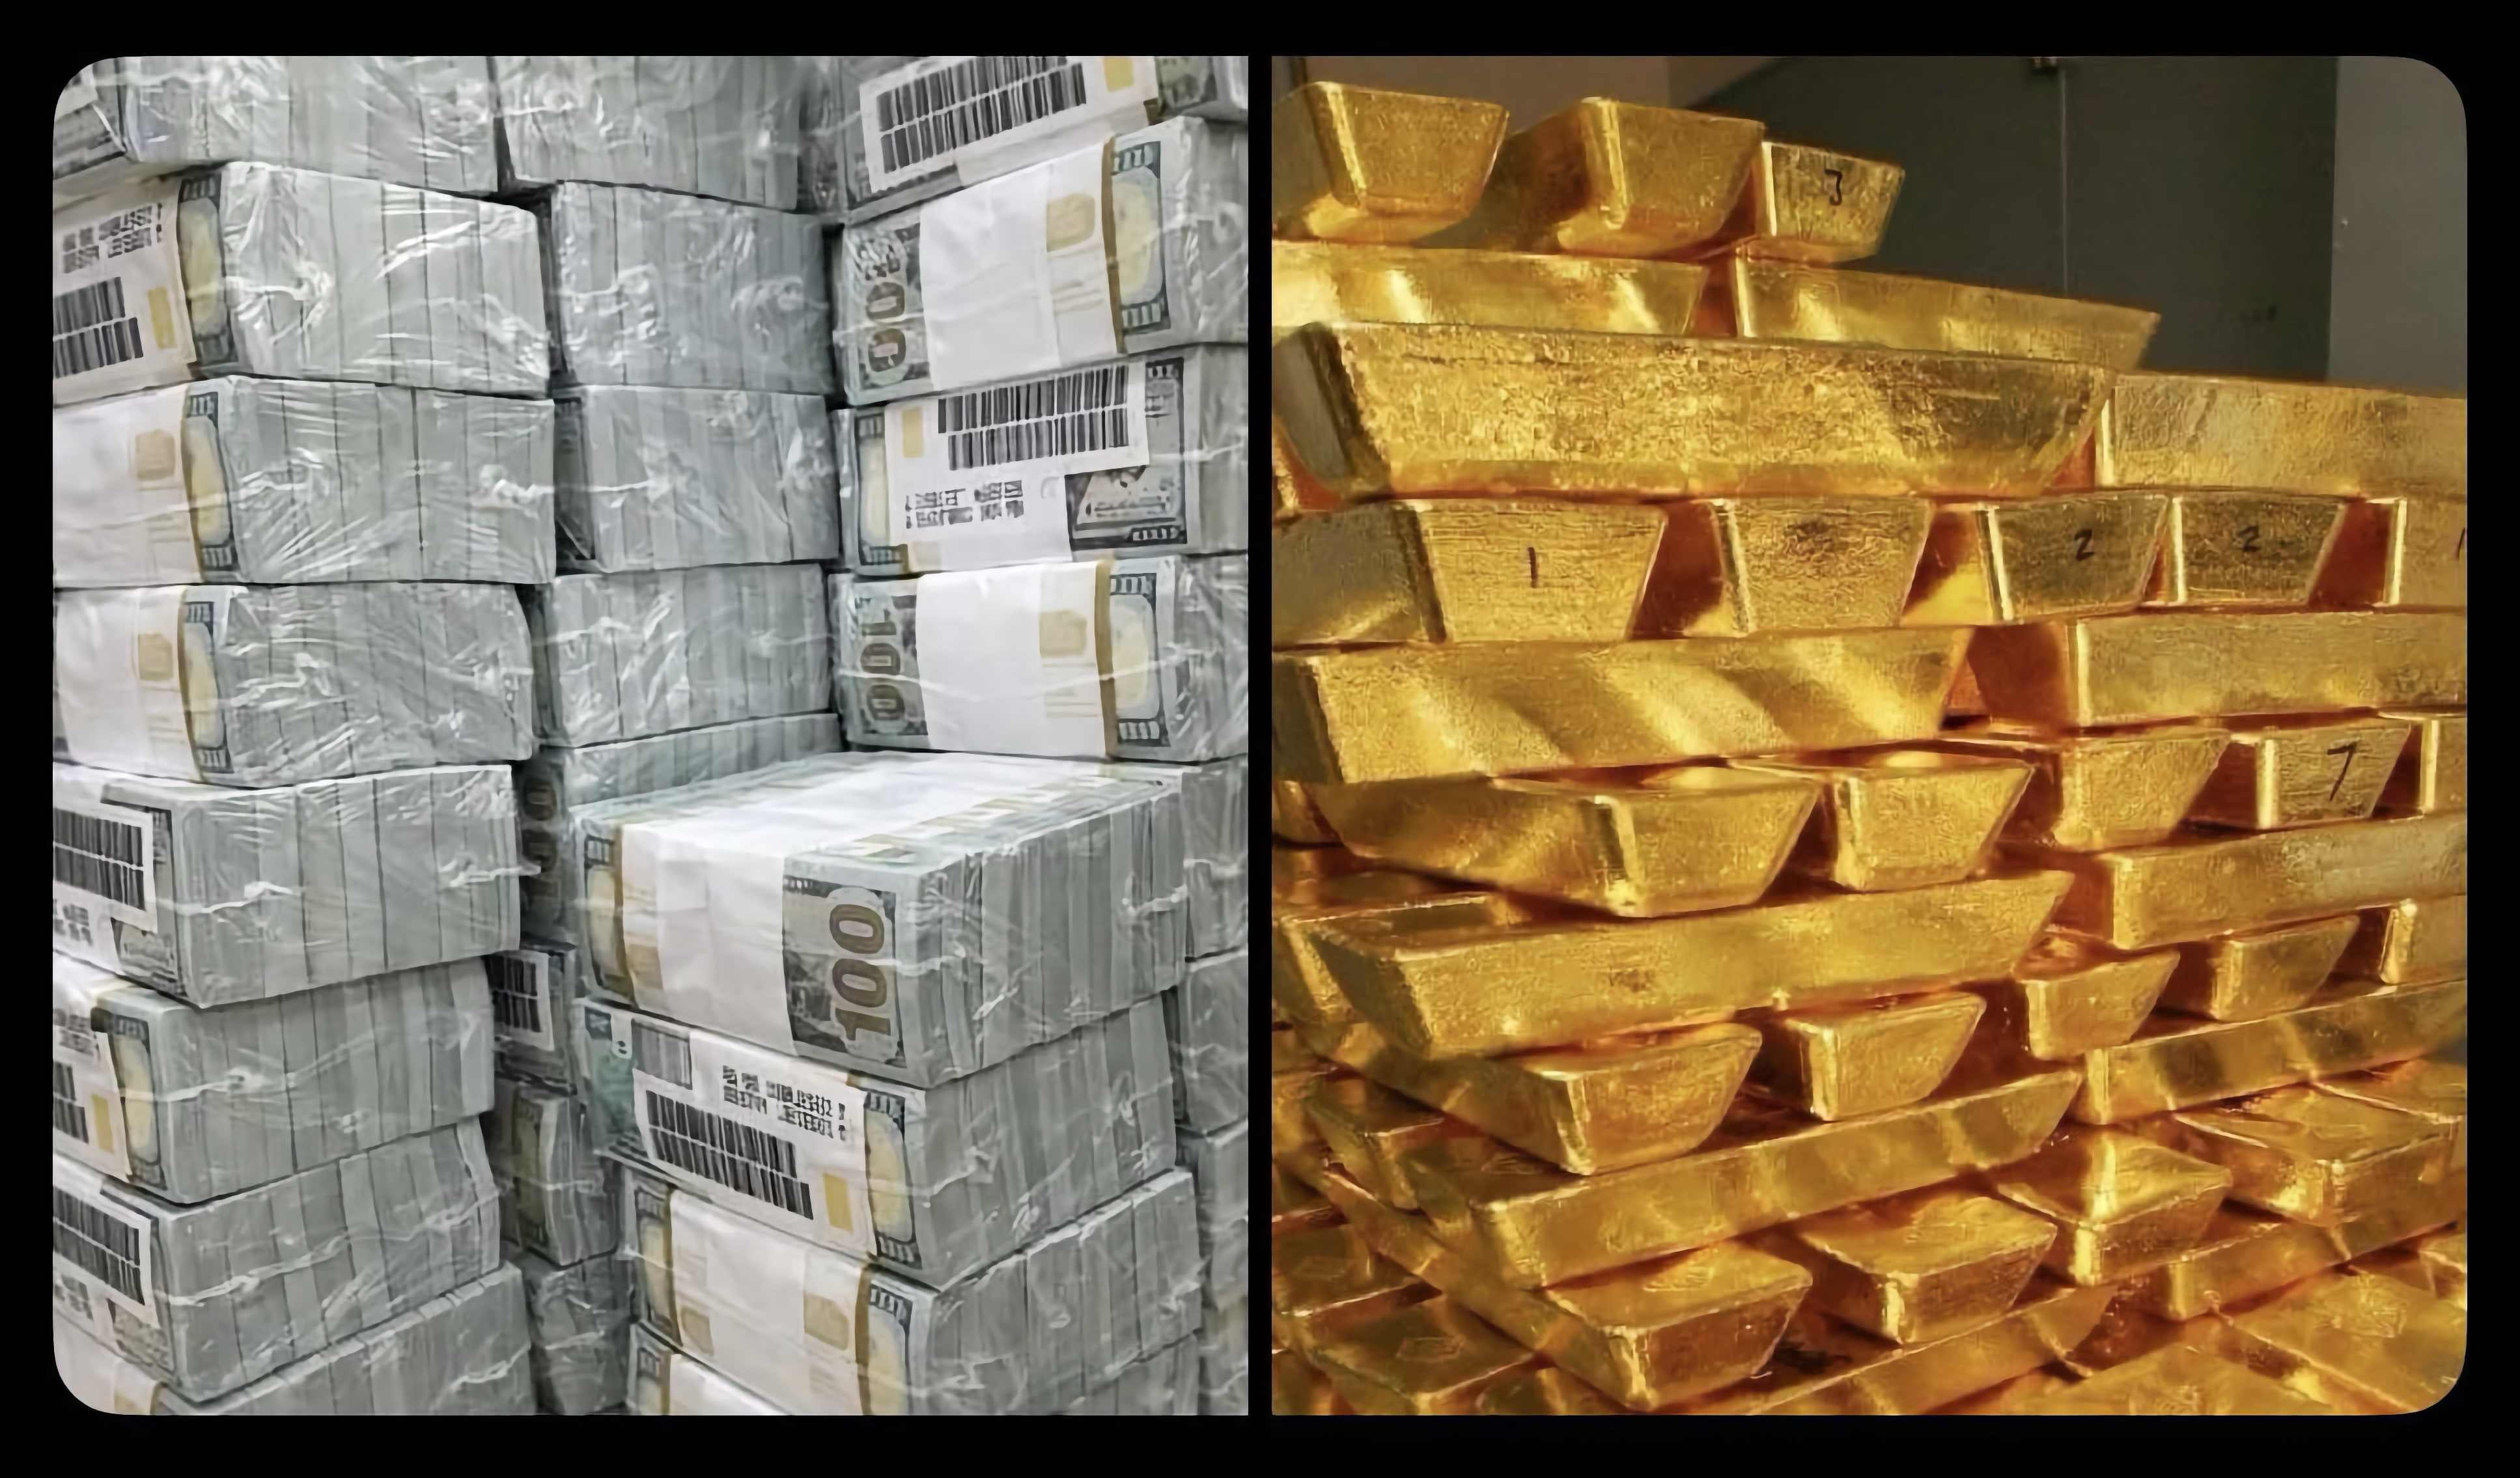
\includegraphics[height=.66\textheight]{DollarGold.jpg}\\
\emph{What would you choose? What would someone else choose?}
\end{block}
\end{frame}

%------------------------------------------------
\begin{frame}{}
\small
Are we modeling risk itself,\\or merely the aspects of \ul{uncertainty} that are easiest to quantify?
\begin{center}
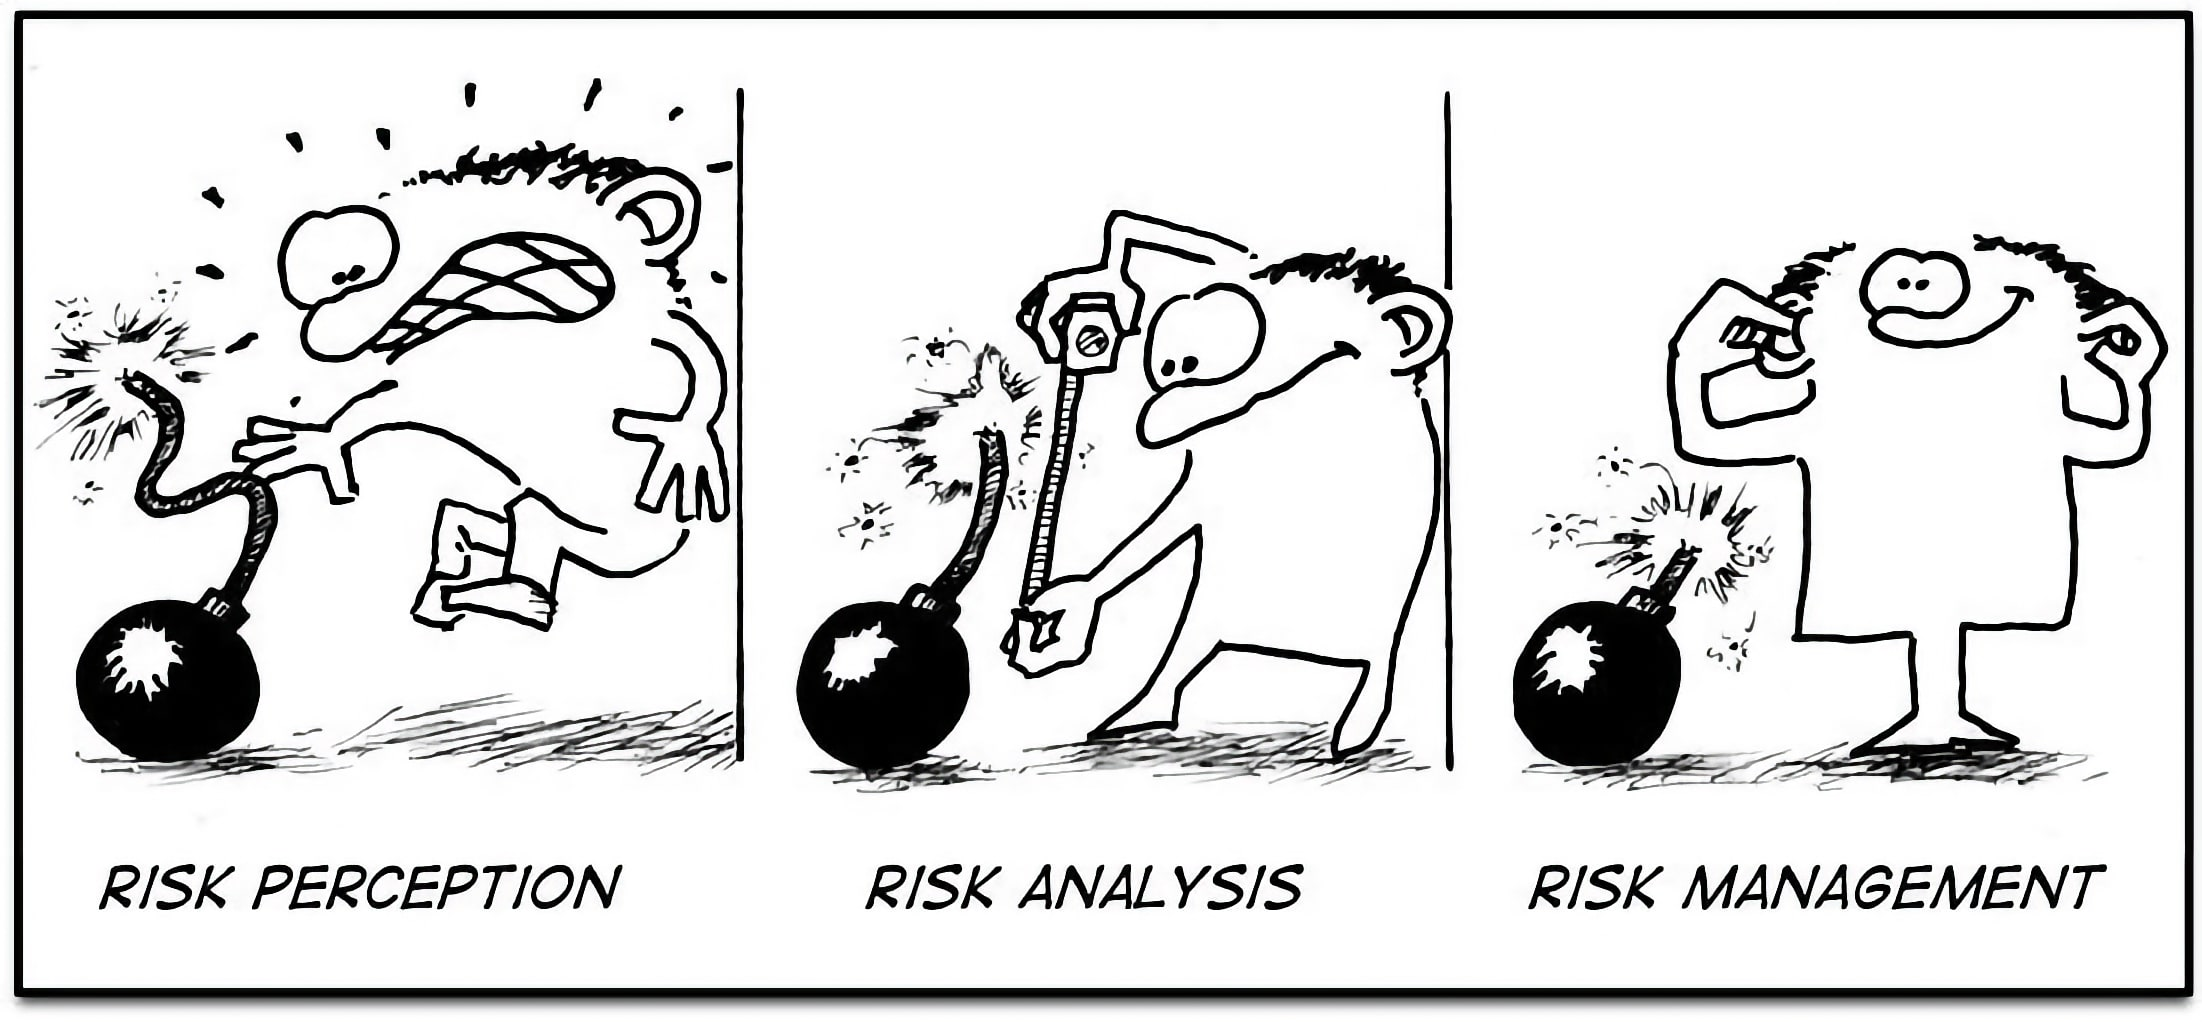
\includegraphics[width=.6\textwidth]{risks.jpg}
\end{center}
\pause
\vocab{Example}:
A flood risk model might estimate: "There is a 2\% annual probability of flooding, with an expected property loss of \$40,000."\\
That is mathematically convenient: \emph{probability x expected loss}.
But it may ignore whether residents trust the model or can afford insurance,
or political leaders delay action, or infrastructure fails under stress.
So the question becomes: \vocab{"Are we modeling the full risk of flooding, or just the measurable part: water levels, probabilities, and dollar losses?"}
\end{frame}

%-----------------------------------------------
\begin{frame}{}
\begin{block}{Alexander Abuabara, PhD}
\begin{itemize}
    \item About me: \url{https://abuabara.github.io}
    \item \textcolor{purple}{\textbf{To be a great teacher ...}}
\end{itemize}
\end{block}
\centering
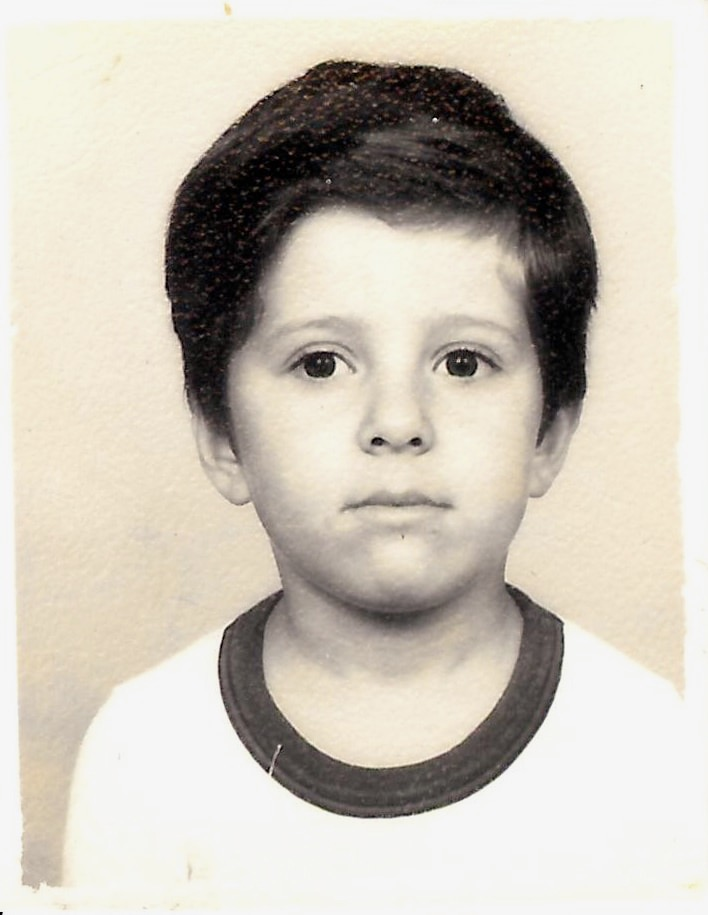
\includegraphics[height=5cm]{abuabara.jpg}
\end{frame}

%-----------------------------------------------
\begin{frame}{}
\begin{itemize}
    \item \textcolor{purple}{\textbf{To be a great teacher ...} that means always learning, adapting, and getting better each and every day.}
    \item \textbf{That you \ul{learn}} concepts, analyze data, pass the class ...\\ \hspace{4.6cm}... and go do great things in life!
\end{itemize}
\centering
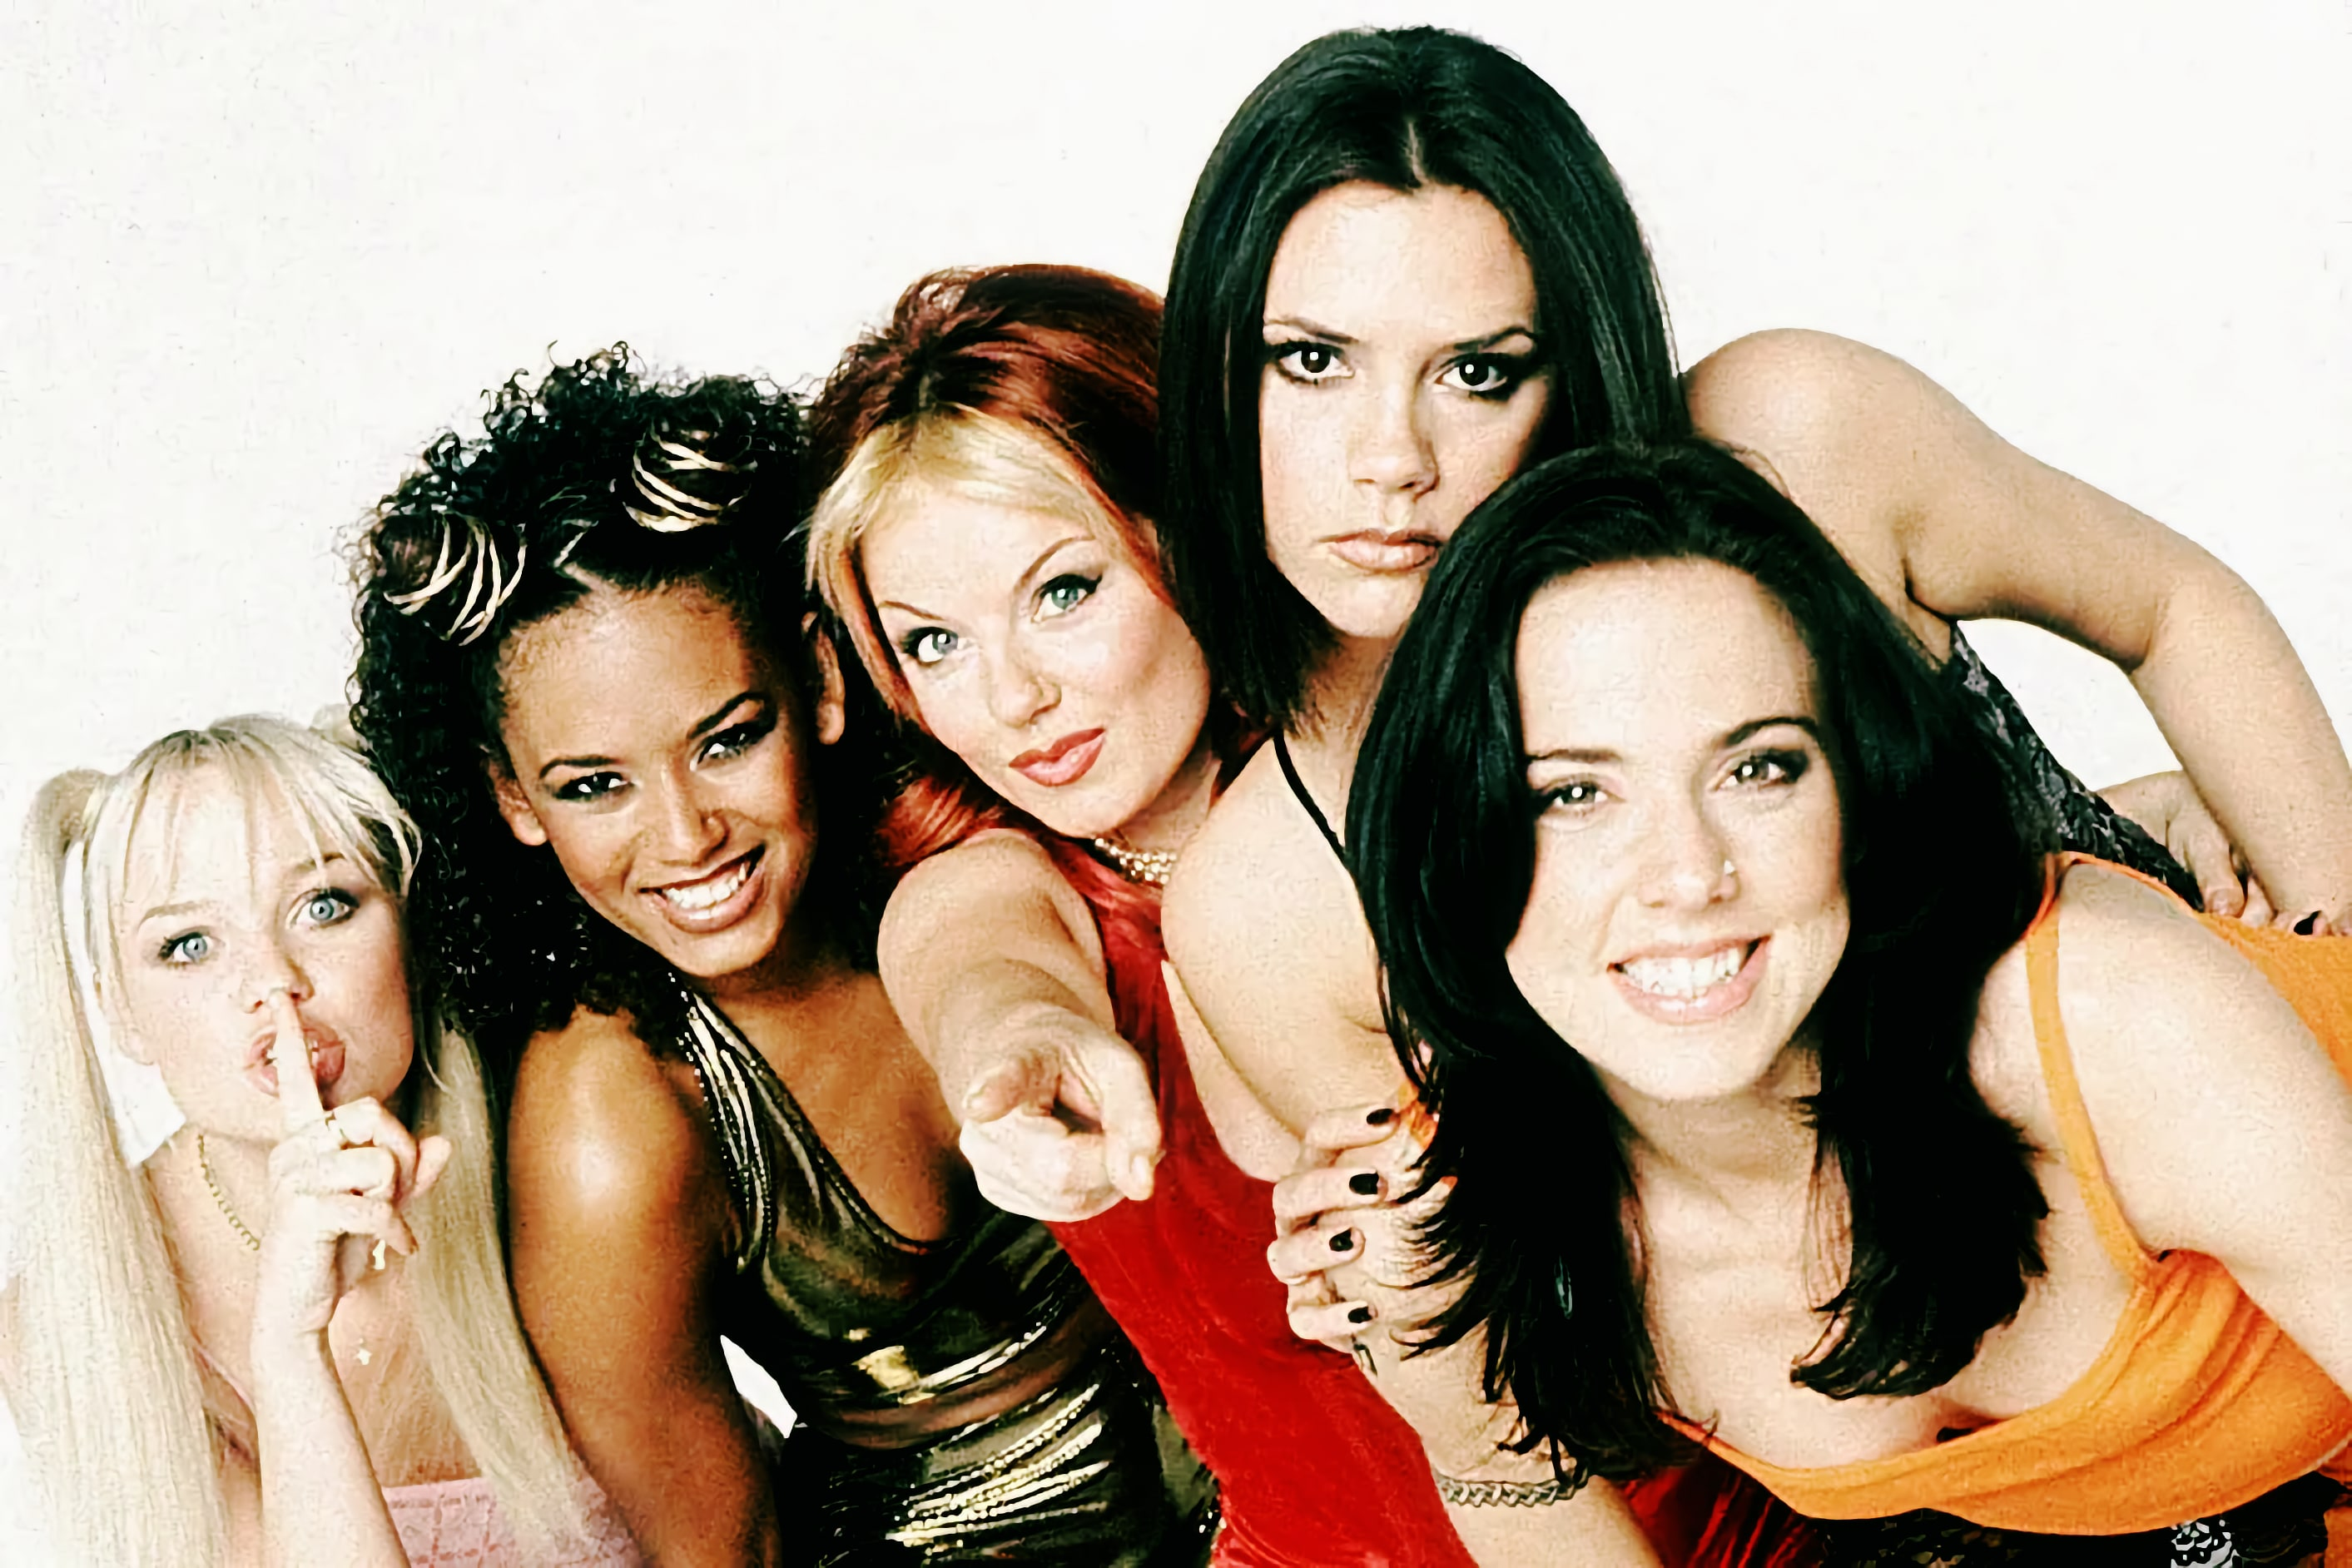
\includegraphics[height=5cm]{spice-girls-spice-world-billboard-1548.jpg}\\
\small{\emph{Yo, I'll tell you what I want, what I really really want}$^*$}\\
\tiny{$^*$Wannabe by Spice Girls}
\end{frame}

%-----------------------------------------------
\begin{frame}{}
\begin{itemize}
    \item At first, it may seem that answers are the most important.
    \item But the real goal is \textbf{to learn how to ASK questions}.
    \item When you can create thoughtful questions about a topic means you truly understand it.
    \item[] \qquad \qquad \qquad 
\includegraphics[height=4cm]{Meme-face-thumbs-up.png}
    \item[] Next: \vocab{Syllabus}!
\end{itemize}
\end{frame}
\end{document}